\chapter{Einstieg in SQL}
\chaptertoc{}
\cleardoubleevenpage

\section{Einführung}
SQL\footnote{SQL = Structured Query Language} ist die auf dem Markt etablierte Manipulations- und Abfragesprache für relationale Datenbankmanagementsysteme. Es kam erstmals mit Oracle V2 1979 auf den Markt und wurde durch die beiden Institute ANSI (1986) und ISO (1987) standardisiert. 1989 wurden die Arbeitsergebnisse der beiden Gremien im \enquote{SQL-89} bzw. \enquote{SQL-1} Standard zusammengefasst. Eine grundlegende Überarbeitung erfolgte 1992 mit dem \enquote{SQL-2} Standard, der auch als \enquote{SQL-92} Standard bezeichnet wird, welcher im Wesentlichen auch heute noch Anwendung findet. Der aktuell gültige SQL-Standard ist der \enquote{SQL-2003} Standard (SQL:2003 ISO/IEC 9075).

\begin{itemize}
    \item \textbf{1989 - SQL-89-Standard, SQL-1-Standard}
          \begin{small}
              \begin{itemize}
                  \item DML (Data Manipulation Language): SELECT, INSERT, UPDATE, DELETE
                  \item DDL (Data Definition Language): Tabellen, Indizes, Sichten, GRANT/REVOKE
                  \item Transaktionen: BEGIN, COMMIT, ROLLBACK
                  \item Cursor
              \end{itemize}
          \end{small}
    \item \textbf{1992 - SQL-92-Standard, SQL-2-Standard}
          \begin{small}
              \begin{itemize}
                  \item DDL (Data Definition Language): BLOB, VARCHAR, DATE, TIME, TIMESTAMP, BOOLEAN
                  \item DML (Data Manipulation Language): INNER- und OUTER-Join, SET-Operatoren
                  \item Transaktionen: SET TRANSACTION
                  \item Cursor
                  \item Constraints
                  \item Systemtabellen
              \end{itemize}
          \end{small}
    \item \textbf{1999 - SQL-99-Standard, SQL-3-Standard}
          \begin{small}
              \begin{itemize}
                  \item DML (Data Manipulation Language): Benutzerdefinierte Datentypen, Rollen
                  \item DDL (Data Definition Language): Rekursive Abfragen
                        \begin{itemize}
                            \item Intermediate Level: CASCADE DELETE
                            \item Full Level: CASCADE UPDATE
                        \end{itemize}
                  \item Constraints: Trigger
                  \item Call Level Interface: ODBC, JDBC, OLE DB
                  \item Persistent Storage Modules: Stored Procedures
              \end{itemize}
          \end{small}
          \clearpage
    \item \textbf{2003 - SQL-2003-Standard}
          \begin{small}
              \begin{itemize}
                  \item DML (Data Manipulation Language): MERGE
                  \item DDL (Data Definition Language): Identitätsattribute
                  \item Schemata: Informations- und Definitions Schema
                  \item SQL/XML: Einbettung von XML in die Datenbank
                  \item Mediums: Zugriff auf externe Daten
              \end{itemize}
          \end{small}
\end{itemize}
Seit Ende der 80er-Jahr wird SQL, in Teilen, von nahezu allen relationalen Datenbankmanagementsystemen unterstützt, wobei jeder Hersteller seine eigenen Erweiterungen, zusätzlich zum Standard einfügt. Dies führt dazu, dass es eine Vielzahl von SQL-Dialekten gibt, welche sehr unterschiedlich sein können.

Die Syntax von SQL ist stark an die englische Sprache angelehnt und somit relativ einfach zu erlernen. Es stellt eine Reihe von Befehlen zur Verfügung, welche sich in vier Kategorien einteilen lassen:
\begin{itemize}
    \item Abfragesprache (Query-Language)
    \item Datenmanipulationssprache (DML Data Manipulation Language)
    \item Datendefinitionssprache (DDL Data Definition Language)
    \item Datenkontrollsprache (DCL Data Control Language)
\end{itemize}
Durch die weitreichende Standardisierung von SQL, ist es möglich Anwendungsprogramme zu erstellen, welche eingeschränkt unabhängig vom verwendeten DBMS sind. Dies gilt zumindest für die Teile des SQL-Standards, die von allen Anbietern implementiert werden.

Im Gegensatz zu Programmiersprachen, wie z. B. Turbo Pascal, C++ oder Java, handelt es sich bei SQL um eine \enquote{Deklarative Programmiersprache}. Dies bedeutet, dass während in einer Sprache, wie C++, der \textit{genaue Weg zur Lösung eines Problems} beschrieben wird, in SQL der Programmierer das \textit{gewünschte Ergebnis so genau wie möglich} beschreiben muss. Den Weg dorthin findet SQL selbst, so dass sich der Programmierer nicht darum kümmern braucht, wie SQL zu seinem Ergebnis kommt.

Problematisch an diesem Ansatz kann sein, dass SQL immer ein Ergebnis liefert, solange die Syntax der Anweisung korrekt ist. Das gefundene Ergebnis muss jedoch nicht unbedingt das Gewollte sein und kann sich, in sehr geringen Details, vom Richtigen unterscheiden, was eine Fehlersuche bzw. das Bemerken eines Fehlers sehr schwierig gestaltet.

In diesem Skript werden Teile der beiden SQL-Dialekte, von Oracle 11g R2 und Microsoft SQL-Server 2008 R2 bzw. SQL Server 2012, anhand von praktischen Beispielen, näher erleutert.
\section{Grundlegende Operationen in SQL}
SQL basiert auf einer Relationalen Algebra. Im Sinne der Datenbanktheorie, ist dies eine formale Sprache, die es ermöglicht, Suchoperationen auf einem relationalen Schema durchzuführen. Mit ihrer Hilfe hat man die Möglichkeit, Relationen zu verknüpfen, zu reduzieren und komplexe Informationen zu ermitteln.

Die Relationale Algebra stellt verschiedene Operationen bereit, welche, mit Hilfe von SQL, umgesetzt werden können.
\begin{itemize}
    \item Mengenoperationen
          \begin{itemize}
              \item Vereinigung (UNION)
              \item Schnittmenge (INTERSECT)
              \item Differenz (MINUS)
          \end{itemize}
    \item Projektion
    \item Selektion
    \item Kreuzprodukt (Kartesisches Produkt)
    \item Join
\end{itemize}
Für diese Unterrichtsunterlage hat die Relationale Algebra nur insofern eine Bedeutung, dass sie die theoretische Grundlage für die Sprache SQL darstellt.
\subsection{Mengenoperationen}
\subsubsection{Die Vereinigung}
Die Vereinigung ist eine Operation, bei der alle Zeilen zweier Relationen zu einer neuen Relation zusammengeführt werden. Dargestellt wird die Vereinigung in der Relationalen Algebra mit: $R_1\cup R_2$ ($R_1$ vereinigt mit $R_2$).

Das folgende Beispiel veranschaulicht die Funktionsweise dieser Mengenoperation. Die beiden Relationen $R_1$ und $R_2$ werden miteinander vereinigt. Als Ergebnis entsteht eine neue Relation, die alle Zeilen der beiden zugrunde gelegten Relationen enthält, mit Ausnahme der Zeilen, welche redundant vorkommen. Dies betrifft hier die Zeile \enquote{1 2 3 4}, in der Relation $R_2$. Eine gleiche Zeile existiert bereits in der Relation $R_1$. Somit wird diese Zeile nur einmal im Ergebnis erscheinen.
\begin{center}
    \begin{small}
        \begin{minipage}[b]{.2\linewidth}
            \begin{center}
                \tablecaption{$R_1$}
                \tablefirsthead{
                    \hline
                    \multicolumn{1}{|c}{\textbf{A}} &
                    \multicolumn{1}{|c}{\textbf{B}} &
                    \multicolumn{1}{|c}{\textbf{C}} &
                    \multicolumn{1}{|c|}{\textbf{D}} \\
                    \hline
                }
                \tabletail{
                    \hline
                }
                \tablelasttail{
                    \hline
                }
                \begin{supertabular}{|c|c|c|c|}
                    \textcolor{red}{1} & \textcolor{red}{2} & \textcolor{red}{3} & \textcolor{red}{4} \\
                    \hline
                    \textcolor{red}{5} & \textcolor{red}{6} & \textcolor{red}{7} & \textcolor{red}{8} \\
                \end{supertabular}
            \end{center}
        \end{minipage}
        \hfil
        \begin{minipage}[b]{.2\linewidth}
            \begin{center}
                \tablecaption{$R_2$}
                \tablefirsthead{
                    \hline
                    \multicolumn{1}{|c}{\textbf{A}} &
                    \multicolumn{1}{|c}{\textbf{B}} &
                    \multicolumn{1}{|c}{\textbf{C}} &
                    \multicolumn{1}{|c|}{\textbf{D}} \\
                    \hline
                }
                \tabletail{
                    \hline
                }
                \tablelasttail{
                    \hline
                }
                \begin{supertabular}{|c|c|c|c|}
                    \textcolor{red}{0} & \textcolor{red}{9} & \textcolor{red}{8} & \textcolor{red}{7} \\
                    \hline
                    \textcolor{red}{6} & \textcolor{red}{5} & \textcolor{red}{4} & \textcolor{red}{3} \\
                    \hline
                    1 & 2 & 3 & 4  \\
                \end{supertabular}
            \end{center}
        \end{minipage}
        \hfil
        \begin{minipage}[b]{.2\linewidth}
            \begin{center}
                \tablecaption{$R_1\cup R_2$}
                \tablefirsthead{
                    \hline
                    \multicolumn{1}{|c}{\textbf{A}} &
                    \multicolumn{1}{|c}{\textbf{B}} &
                    \multicolumn{1}{|c}{\textbf{C}} &
                    \multicolumn{1}{|c|}{\textbf{D}} \\
                    \hline
                }
                \tabletail{
                    \hline
                }
                \tablelasttail{
                    \hline
                }
                \begin{supertabular}{|c|c|c|c|}
                    \textcolor{red}{1} & \textcolor{red}{2} & \textcolor{red}{3} & \textcolor{red}{4} \\
                    \hline
                    \textcolor{red}{5} & \textcolor{red}{6} & \textcolor{red}{7} & \textcolor{red}{8} \\
                    \hline
                    \textcolor{red}{0} & \textcolor{red}{9} & \textcolor{red}{8} & \textcolor{red}{7} \\
                    \hline
                    \textcolor{red}{6} & \textcolor{red}{5} & \textcolor{red}{4} & \textcolor{red}{3} \\
                \end{supertabular}
            \end{center}
        \end{minipage}
    \end{small}
\end{center}
\begin{merke}
    Redundante Zeilen werden bei der Vereinigung zweier Relationen $R_1$ und $R_2$ aus dem Ergebnis entfernt!
\end{merke}
\subsubsection{Die Schnittmenge}
Die Schnittmenge enthält als Ergebnis nur die Zeilen, die in den beiden Relationen $R_1$ und $R_2$ identisch sind. Die Darstellung erfolgt in der Relationalen Algebra mit: $R_1\cap R_2$ ($R_1$ geschnitten mit $R_2$).

\begin{center}
    \begin{small}
        \begin{minipage}[b]{.2\linewidth}
            \begin{center}
                \tablecaption{$R_1$}
                \tablefirsthead{
                    \hline
                    \multicolumn{1}{|c}{\textbf{A}} &
                    \multicolumn{1}{|c}{\textbf{B}} &
                    \multicolumn{1}{|c}{\textbf{C}} &
                    \multicolumn{1}{|c|}{\textbf{D}} \\
                    \hline
                }
                \tabletail{
                    \hline
                }
                \tablelasttail{
                    \hline
                }
                \begin{supertabular}{|c|c|c|c|}
                    \textcolor{red}{1} & \textcolor{red}{2} & \textcolor{red}{3} & \textcolor{red}{4} \\
                    \hline
                    5 & 6 & 7 & 8 \\
                \end{supertabular}
            \end{center}
        \end{minipage}
        \hfil
        \begin{minipage}[b]{.2\linewidth}
            \begin{center}
                \tablecaption{$R_2$}
                \tablefirsthead{
                    \hline
                    \multicolumn{1}{|c}{\textbf{A}} &
                    \multicolumn{1}{|c}{\textbf{B}} &
                    \multicolumn{1}{|c}{\textbf{C}} &
                    \multicolumn{1}{|c|}{\textbf{D}} \\
                    \hline
                }
                \tabletail{
                    \hline
                }
                \tablelasttail{
                    \hline
                }
                \begin{supertabular}{|c|c|c|c|}
                    0 & 9 & 8 & 7 \\
                    \hline
                    6 & 5 & 4 & 3 \\
                    \hline
                    \textcolor{red}{1} & \textcolor{red}{2} & \textcolor{red}{3} & \textcolor{red}{4} \\
                \end{supertabular}
            \end{center}
        \end{minipage}
        \hfil
        \begin{minipage}[b]{.2\linewidth}
            \begin{center}
                \tablecaption{$R_1\cap R_2$}
                \tablefirsthead{
                    \hline
                    \multicolumn{1}{|c}{\textbf{A}} &
                    \multicolumn{1}{|c}{\textbf{B}} &
                    \multicolumn{1}{|c}{\textbf{C}} &
                    \multicolumn{1}{|c|}{\textbf{D}} \\
                    \hline
                }
                \tabletail{
                    \hline
                }
                \tablelasttail{
                    \hline
                }
                \begin{supertabular}{|c|c|c|c|}
                    \textcolor{red}{1} & \textcolor{red}{2} & \textcolor{red}{3} & \textcolor{red}{4} \\
                \end{supertabular}
            \end{center}
        \end{minipage}
    \end{small}
\end{center}
Da in diesem Beispiel nur die Zeile \enquote{1 2 3 4} in beiden Relationen $R_1$ und $R_2$ vorhanden ist, wird nur diese in der Ergebnisrelation $R_1\cap R_2$ abgebildet.
\subsubsection{Die Differenz}
Die Differenz zweier Relationen $R_1$ und $R_2$ entspricht den Zeilen, die nur in der linken der beiden Relationen vorkommen. D. h., die Differenz ist, wie in der Arithmetik auch, nicht kommutativ ($R_1 \setminus R_2 \neq R_2 \setminus R_1$).

\begin{center}
    \begin{small}
        \begin{minipage}[b]{.2\linewidth}
            \begin{center}
                \tablecaption{$R_1$}
                \tablefirsthead{
                    \hline
                    \multicolumn{1}{|c}{\textbf{A}} &
                    \multicolumn{1}{|c}{\textbf{B}} &
                    \multicolumn{1}{|c}{\textbf{C}} &
                    \multicolumn{1}{|c|}{\textbf{D}} \\
                    \hline
                }
                \tabletail{
                    \hline
                }
                \tablelasttail{
                    \hline
                }
                \begin{supertabular}{|c|c|c|c|}
                    1 & 2 & 3 & 4 \\
                    \hline
                    \textcolor{red}{5} & \textcolor{red}{6} & \textcolor{red}{7} & \textcolor{red}{8} \\
                \end{supertabular}
            \end{center}
        \end{minipage}
        \hfil
        \begin{minipage}[b]{.2\linewidth}
            \begin{center}
                \tablecaption{$R_2$}
                \tablefirsthead{
                    \hline
                    \multicolumn{1}{|c}{\textbf{A}} &
                    \multicolumn{1}{|c}{\textbf{B}} &
                    \multicolumn{1}{|c}{\textbf{C}} &
                    \multicolumn{1}{|c|}{\textbf{D}} \\
                    \hline
                }
                \tabletail{
                    \hline
                }
                \tablelasttail{
                    \hline
                }
                \begin{supertabular}{|c|c|c|c|}
                    \textcolor{blue}{0} & \textcolor{blue}{9} & \textcolor{blue}{8} & \textcolor{blue}{7} \\
                    \hline
                    \textcolor{blue}{6} & \textcolor{blue}{5} & \textcolor{blue}{4} & \textcolor{blue}{3} \\
                    \hline
                    1 & 2 & 3 & 4  \\
                \end{supertabular}
            \end{center}
        \end{minipage}
        \hfil
        \begin{minipage}[b]{.2\linewidth}
            \begin{center}
                \tablecaption{$R_1 \setminus R_2$}
                \tablefirsthead{
                    \hline
                    \multicolumn{1}{|c}{\textbf{A}} &
                    \multicolumn{1}{|c}{\textbf{B}} &
                    \multicolumn{1}{|c}{\textbf{C}} &
                    \multicolumn{1}{|c|}{\textbf{D}} \\
                    \hline
                }
                \tabletail{
                    \hline
                }
                \tablelasttail{
                    \hline
                }
                \begin{supertabular}{|c|c|c|c|}
                    \textcolor{red}{5} & \textcolor{red}{6} & \textcolor{red}{7} & \textcolor{red}{8} \\
                \end{supertabular}
            \end{center}
        \end{minipage}
        \hfil
        \begin{minipage}[b]{.2\linewidth}
            \begin{center}
                \tablecaption{$R_2 \setminus R_1$}
                \tablefirsthead{
                    \hline
                    \multicolumn{1}{|c}{\textbf{A}} &
                    \multicolumn{1}{|c}{\textbf{B}} &
                    \multicolumn{1}{|c}{\textbf{C}} &
                    \multicolumn{1}{|c|}{\textbf{D}} \\
                    \hline
                }
                \tabletail{
                    \hline
                }
                \tablelasttail{
                    \hline
                }
                \begin{supertabular}{|c|c|c|c|}
                    \textcolor{blue}{0} & \textcolor{blue}{9} & \textcolor{blue}{8} & \textcolor{blue}{7} \\
                    \hline
                    \textcolor{blue}{6} & \textcolor{blue}{5} & \textcolor{blue}{4} & \textcolor{blue}{3} \\
                \end{supertabular}
            \end{center}
        \end{minipage}
    \end{small}
\end{center}
\subsection{Die Projektion}
Die Projektion wählt Attribute aus einer Relation (Spalten aus einer Tabelle) aus, weshalb sie auch als \textit{Attributbeschränkung} bezeichnet wird. Es ist dabei egal, ob alle Attribute oder nur eine Teilmenge der Attributmenge ausgewählt wird. In der Relationalen Algebra wird die Projektion mit $\pi_\beta(R_1)$ ausgedrückt, wobei $\beta$ die Liste der gewählten Attribute bezeichnet. Hierzu ein paar Beispiele:
\begin{center}
    \begin{small}
        \begin{minipage}[b]{.19\linewidth}
            \begin{center}
                \tablecaption{$R_1$}
                \tablefirsthead{
                    \hline
                    \multicolumn{1}{|c}{\textbf{A}} &
                    \multicolumn{1}{|c}{\textbf{B}} &
                    \multicolumn{1}{|c}{\textbf{C}} &
                    \multicolumn{1}{|c|}{\textbf{D}} \\
                    \hline
                }
                \tabletail{
                    \hline
                }
                \tablelasttail{
                    \hline
                }
                \begin{supertabular}{|c|c|c|c|}
                    1 & 2 & 3 & 4 \\
                    \hline
                    5 & 6 & 7 & 8 \\
                \end{supertabular}
            \end{center}
        \end{minipage}
        \hfil
        \begin{minipage}[b]{.25\linewidth}
            \begin{center}
                \tablecaption{$\pi_{(A,B)}(R_1)$}
                \tablefirsthead{
                    \hline
                    \multicolumn{1}{|c}{\textbf{A}} &
                    \multicolumn{1}{|c|}{\textbf{B}} \\
                    \hline
                }
                \tabletail{
                    \hline
                }
                \tablelasttail{
                    \hline
                }
                \begin{supertabular}{|c|c|}
                    1 & 2 \\
                    \hline
                    5 & 6 \\
                \end{supertabular}
            \end{center}
        \end{minipage}
        \hfil
        \begin{minipage}[b]{.19\linewidth}
            \begin{center}
                \tablecaption{$\pi_A(R_1)$}
                \tablefirsthead{
                    \hline
                    \multicolumn{1}{|c|}{\textbf{A}} \\
                    \hline
                }
                \tabletail{
                    \hline
                }
                \tablelasttail{
                    \hline
                }
                \begin{supertabular}{|c|}
                    1 \\
                    \hline
                    5 \\
                \end{supertabular}
            \end{center}
        \end{minipage}
        \hfil
        \begin{minipage}[b]{.19\linewidth}
            \begin{center}
                \tablecaption{$\pi_*(R_1)$}
                \tablefirsthead{
                    \hline
                    \multicolumn{1}{|c}{\textbf{A}} &
                    \multicolumn{1}{|c}{\textbf{B}} &
                    \multicolumn{1}{|c}{\textbf{C}} &
                    \multicolumn{1}{|c|}{\textbf{D}} \\
                    \hline
                }
                \tabletail{
                    \hline
                }
                \tablelasttail{
                    \hline
                }
                \begin{supertabular}{|c|c|c|c|}
                    1 & 2 & 3 & 4 \\
                    \hline
                    5 & 6 & 7 & 8 \\
                \end{supertabular}
            \end{center}
        \end{minipage}
    \end{small}
\end{center}
\subsection{Die Selektion}
\label{dieselektion}
Die Selektion ermöglicht es ausgewählte Zeilen aus einer Relation in das Ergebnis aufzunehmen. Nicht erwünschte Zeilen werden einfach ausgeblendet. Dies geschieht mit einem \enquote{Selektionsausdruck}, einer einfachen Bedingung, die für jede einzelne Zeile geprüft wird. Mathematisch wird die Selektion als $\sigma_{Ausdruck}(R)$ dargestellt. $\sigma$ (sigma) steht für Selektion.

\begin{center}
    \begin{small}
        \begin{minipage}[b]{.2\linewidth}
            \begin{center}
                \tablecaption{$R_1$}
                \tablefirsthead{
                    \hline
                    \multicolumn{1}{|c}{\textbf{A}} &
                    \multicolumn{1}{|c}{\textbf{B}} &
                    \multicolumn{1}{|c}{\textbf{C}} &
                    \multicolumn{1}{|c|}{\textbf{D}} \\
                    \hline
                }
                \tabletail{
                    \hline
                }
                \tablelasttail{
                    \hline
                }
                \begin{supertabular}{|c|c|c|c|}
                    1 & 2 & 3 & 4 \\
                    \hline
                    5 & 6 & 7 & 8 \\
                    \hline
                    9 & 0 & 1 & 2 \\
                    \hline
                    3 & 4 & 5 & 6 \\
                    \hline
                    7 & 8 & 9 & 0 \\
                \end{supertabular}
            \end{center}
        \end{minipage}
    \end{small}
\end{center}

\begin{center}
    \begin{small}
        \begin{minipage}[b]{.3\linewidth}
            \begin{center}
                \tablecaption{$\sigma_{(A = 3)}\pi_{(A,B)}(R_1)$}
                \tablefirsthead{
                    \hline
                    \multicolumn{1}{|c}{\textbf{A}} &
                    \multicolumn{1}{|c|}{\textbf{B}} \\
                    \hline
                }
                \tabletail{
                    \hline
                }
                \tablelasttail{
                    \hline
                }
                \begin{supertabular}{|c|c|}
                    3 & 4 \\
                \end{supertabular}
            \end{center}
        \end{minipage}
        \hfil
        \begin{minipage}[b]{.3\linewidth}
            \begin{center}
                \tablecaption{$\sigma_{(B \geq 4)}\pi_{(A,B,C)}(R_1)$}
                \tablefirsthead{
                    \hline
                    \multicolumn{1}{|c}{\textbf{A}} &
                    \multicolumn{1}{|c}{\textbf{B}} &
                    \multicolumn{1}{|c|}{\textbf{C}} \\
                    \hline
                }
                \tabletail{
                    \hline
                }
                \tablelasttail{
                    \hline
                }
                \begin{supertabular}{|c|c|c|}
                    5 & 6 & 7 \\
                    \hline
                    3 & 4 & 5 \\
                    \hline
                    7 & 8 & 9 \\
                \end{supertabular}
            \end{center}
        \end{minipage}
        \hfil
        \begin{minipage}[b]{.3\linewidth}
            \begin{center}
                \tablecaption{$\sigma_{(A > 2\wedge B \geq 4)}\pi_*(R_1)$}
                \tablefirsthead{
                    \hline
                    \multicolumn{1}{|c}{\textbf{A}} &
                    \multicolumn{1}{|c}{\textbf{B}} &
                    \multicolumn{1}{|c}{\textbf{C}} &
                    \multicolumn{1}{|c|}{\textbf{D}} \\
                    \hline
                }
                \tabletail{
                    \hline
                }
                \tablelasttail{
                    \hline
                }
                \begin{supertabular}{|c|c|c|c|}
                    \hline
                    5 & 6 & 7 & 8 \\
                    \hline
                    3 & 4 & 5 & 6 \\
                    \hline
                    7 & 8 & 9 & 0 \\
                \end{supertabular}
            \end{center}
        \end{minipage}
    \end{small}
\end{center}

Es ist möglich, einen Selektionsausdruck zu definieren, der eine leere Menge $\oslash$ zum Ergebnis hat. Dies wäre z. B. bei folgendem Ausdruck der Fall: $\sigma_{(A=4)}(\pi_*(R_1))$. Da in der Spalte \identifier{A} in keiner Zeile der Wert 4 vorkommt, ist das Ergebnis eine leere Menge.
\subsection{Kartesisches Produkt}
Das Kartesische Produkt $R_1 \times R_2$ entspricht der Multiplikation aller Zeilen zweier Relationen $R_1$ und $R_2$, sofern alle Attribute unterschiedlich sind. Daraus folgt, dass die Resultatrelation die Kombination aller Zeilen aus $R_1$ und $R_2$ umfasst.

\begin{center}
    \begin{small}
        \begin{minipage}[b]{.2\linewidth}
            \begin{center}
                \tablecaption{$R_1$}
                \tablefirsthead{
                    \hline
                    \multicolumn{1}{|c}{\textbf{A}} &
                    \multicolumn{1}{|c|}{\textbf{B}} \\
                    \hline
                }
                \tabletail{
                    \hline
                }
                \tablelasttail{
                    \hline
                }
                \begin{supertabular}{|c|c|c|c|}
                    1 & 2  \\
                    \hline
                    5 & 6  \\
                \end{supertabular}
            \end{center}
        \end{minipage}
        \hfil
        \begin{minipage}[b]{.2\linewidth}
            \begin{center}
                \tablecaption{$R_2$}
                \tablefirsthead{
                    \hline
                    \multicolumn{1}{|c}{\textbf{C}} &
                    \multicolumn{1}{|c}{\textbf{D}} &
                    \multicolumn{1}{|c}{\textbf{E}} &
                    \multicolumn{1}{|c|}{\textbf{F}} \\
                    \hline
                }
                \tabletail{
                    \hline
                }
                \tablelasttail{
                    \hline
                }
                \begin{supertabular}{|c|c|c|c|}
                    0 & 9 & 8 & 7 \\
                    \hline
                    6 & 5 & 4 & 3 \\
                    \hline
                    1 & 2 & 3 & 4  \\
                \end{supertabular}
            \end{center}
        \end{minipage}
        \hfil
        \begin{minipage}[b]{.3\linewidth}
            \begin{center}
                \tablecaption{$R_1\times R_2$}
                \tablefirsthead{
                    \hline
                    \multicolumn{1}{|c}{\textbf{A}} &
                    \multicolumn{1}{|c}{\textbf{B}} &
                    \multicolumn{1}{|c}{\textbf{C}} &
                    \multicolumn{1}{|c}{\textbf{D}} &
                    \multicolumn{1}{|c}{\textbf{E}} &
                    \multicolumn{1}{|c|}{\textbf{F}} \\
                    \hline
                }
                \tabletail{
                    \hline
                }
                \tablelasttail{
                    \hline
                }
                \begin{supertabular}{|c|c|c|c|c|c|}
                    1 & 2 & 0 & 9 & 8 & 7 \\
                    \hline
                    1 & 2 & 6 & 5 & 4 & 3 \\
                    \hline
                    1 & 2 & 1 & 2 & 3 & 4 \\
                    \hline
                    5 & 6 & 0 & 9 & 8 & 7 \\
                    \hline
                    5 & 6 & 6 & 5 & 4 & 3 \\
                    \hline
                    5 & 6 & 1 & 2 & 3 & 4 \\
                \end{supertabular}
            \end{center}
        \end{minipage}
    \end{small}
\end{center}
\subsection{Die Join-Operation im Allgemeinen}
Das Wort Join bezeichnet zu deutsch einen Verbund. Im Sinne der Relationalen Algebra ist das der Verbund der beiden hintereinander ausgeführten Operationen \enquote{Kartesisches Produkt} und \enquote{Selektion}. Der Selektionsausdruck hat dabei die Form: $R_1\theta R_2$, wobei $\theta$ (theta) einen geeigneten Vergleichsoperator ($=,\neq,>,<$ u. ä.) darstellt.

Die Relationale Algebra definiert den Join wie folgt:

$R_1\bowtie _{Ausdruck} R_2 := \{r_1\cup r_2 | r_1\in R_1 \wedge r_2\in R_2 \wedge Ausdruck\}$
\clearpage

Bedeutung:
\begin{itemize}
    \item \textbf{$R_1\bowtie _{Ausdruck} R_2$}: Verbund der beiden Relation $R_1$ und $R_2$
    \item \textbf{$r_1\cup r_2$}: Vereinigung aller Zeilen aus $R_1$ und $R_2$ (Kreuzprodukt)
    \item \textbf{$r_1\in R_1$}: $r_1$ ist eine Zeile aus der Relation $R_1$
    \item \textbf{$r_2\in R_2$}: $r_2$ ist eine Zeile aus der Relation $R_2$
    \item \textbf{$\wedge$}: UND-Verknüpfung
\end{itemize}

Aus diesem Ausdruck lässt sich die folgende Formel ableiten:

$R_1\bowtie _{Ausdruck} R_2 := \sigma_{Ausdruck}(R_1 \times R_2)$
\subsection{Inner-Joins}
Inner-Joins stellen die am häufigsten benötigte Form der Joins dar, so dass man hier von der \enquote{Standardform eines Joins} sprechen könnte. Bei dieser Form des Joins wird das Kartesische Produkt zweier Relationen $R_1$ und $R_2$ gebildet und anschließend werden alle Zeilen eliminiert, die nicht der Join-Bedingung, auch Join-Prädikat genannt, genügen.

Es gibt zwei Unterarten des Inner-Join, den \enquote{Equi-Join} und den \enquote{Non-Equi-Join}.
\subsubsection{Equi-Join}
Der Equi-Join ist eine spezielle Form des Inner-Join, der dadurch zustande kommt, dass im Join-Prädikat der Operator $=$ als Vergleichsoperator genutzt wird. Nur dann handelt es sich um einen Equi-Join.

$\pi _{(R_1.A, R_1.B,R_2.C)}(R_1\bowtie _{(R_1.A=R_2.A)} R_2 := \sigma _{(R_1.A=R_2.A)}(R_1 \times R_2))$
\clearpage
\begin{center}
    \begin{small}
        \begin{minipage}[b]{.2\linewidth}
            \begin{center}
                \tablecaption{$R_1$}
                \tablefirsthead{
                    \hline
                    \multicolumn{1}{|c}{\textbf{A}} &
                    \multicolumn{1}{|c}{\textbf{B}} &
                    \multicolumn{1}{|c}{\textbf{C}} &
                    \multicolumn{1}{|c|}{\textbf{D}} \\
                    \hline
                }
                \tabletail{
                    \hline
                }
                \tablelasttail{
                    \hline
                }
                \begin{supertabular}{|c|c|c|c|}
                    \colorbox{lightblue}{\textcolor{red}{1}} & \textcolor{red}{2} & 3 & 4 \\
                    \hline
                    5 & 6 & 7 & 8 \\
                    \hline
                    \colorbox{lightblue}{\textcolor{red}{9}} & \textcolor{red}{0} & 1 & 2 \\
                    \hline
                    3 & 4 & 5 & 6 \\
                    \hline
                    7 & 8 & 9 & 0 \\
                \end{supertabular}
            \end{center}
        \end{minipage}
        \hfil
        \begin{minipage}[b]{.2\linewidth}
            \begin{center}
                \tablecaption{$R_2$}
                \tablefirsthead{
                    \hline
                    \multicolumn{1}{|c}{\textbf{A}} &
                    \multicolumn{1}{|c}{\textbf{B}} &
                    \multicolumn{1}{|c}{\textbf{C}} &
                    \multicolumn{1}{|c|}{\textbf{D}} \\
                    \hline
                }
                \tabletail{
                    \hline
                }
                \tablelasttail{
                    \hline
                }
                \begin{supertabular}{|c|c|c|c|}
                    \colorbox{lightblue}{9} & 8 & \textcolor{red}{7} & 6 \\
                    \hline
                    4 & 5 & 2 & 3 \\
                    \hline
                    \colorbox{lightblue}{1} & 0 & \textcolor{red}{9} & 8 \\
                    \hline
                    6 & 4 & 5 & 7 \\
                    \hline
                    0 & 1 & 2 & 3 \\
                \end{supertabular}
            \end{center}
        \end{minipage}

        \begin{minipage}[b]{.3\linewidth}
            \begin{center}
                \tablecaption{$R_1\bowtie R_2$}
                \tablefirsthead{
                    \hline
                    \multicolumn{1}{|c}{\textbf{R1.A}} &
                    \multicolumn{1}{|c}{\textbf{R1.B}} &
                    \multicolumn{1}{|c|}{\textbf{R2.C}} \\
                    \hline
                }
                \tabletail{
                    \hline
                }
                \tablelasttail{
                    \hline
                }
                \begin{supertabular}{|c|c|c|}
                    \colorbox{lightblue}{\textcolor{red}{1}} & \textcolor{red}{2} & \textcolor{red}{9} \\
                    \hline
                    \colorbox{lightblue}{\textcolor{red}{9}} & \textcolor{red}{0} & \textcolor{red}{7} \\
                \end{supertabular}
            \end{center}
        \end{minipage}
    \end{small}
\end{center}
In diesem Beispiel werden die Attributwerte der Spalten $R_1.A$ und $R_2.A$ miteinander verglichen und nur dort, wo eine Übereinstimmung gefunden wird, wird diese Zeile in die Ergebnisrelation aufgenommen.
\subsubsection{Non-Equi-Join}
Beim Non-Equi-Join handelt es sich um das Gegenteil zum Equi-Join. Sobald im Join-Prädikat nicht der $=$-Operator genutzt wird, handelt es sich um einen Non-Equi-Join.

$\pi _{R_2.*}(R_1\bowtie _{(R_1.A > R_2.A\wedge R_1.B < R_2.B)} R_2)$

\begin{center}
    \begin{small}
        \begin{minipage}[b]{.2\linewidth}
            \begin{center}
                \tablecaption{$R_1$}
                \tablefirsthead{
                    \hline
                    \multicolumn{1}{|c}{\textbf{A}} &
                    \multicolumn{1}{|c}{\textbf{B}} &
                    \multicolumn{1}{|c}{\textbf{C}} &
                    \multicolumn{1}{|c|}{\textbf{D}} \\
                    \hline
                }
                \tabletail{
                    \hline
                }
                \tablelasttail{
                    \hline
                }
                \begin{supertabular}{|c|c|c|c|}
                    1 & 2 & 3 & 4 \\
                    \hline
                    5 & 6 & 7 & 8 \\
                    \hline
                    \colorbox{lightblue}{9} & \colorbox{lightblue}{0} & 1 & 2 \\
                    \hline
                    3 & 4 & 5 & 6 \\
                    \hline
                    7 & 8 & 9 & 0 \\
                \end{supertabular}
            \end{center}
        \end{minipage}
        \hfil
        \begin{minipage}[b]{.2\linewidth}
            \begin{center}
                \tablecaption{$R_2$}
                \tablefirsthead{
                    \hline
                    \multicolumn{1}{|c}{\textbf{A}} &
                    \multicolumn{1}{|c}{\textbf{B}} &
                    \multicolumn{1}{|c}{\textbf{C}} &
                    \multicolumn{1}{|c|}{\textbf{D}} \\
                    \hline
                }
                \tabletail{
                    \hline
                }
                \tablelasttail{
                    \hline
                }
                \begin{supertabular}{|c|c|c|c|}
                    9 & 8 & 7 & 6 \\
                    \hline
                    5 & 4 & 3 & 2 \\
                    \hline
                    1 & 0 & 9 & 8 \\
                    \hline
                    \colorbox{lightblue}{7} & \colorbox{lightblue}{6} & 5 & 4 \\
                    \hline
                    \colorbox{lightblue}{3} & \colorbox{lightblue}{2} & 1 & 0 \\
                \end{supertabular}
            \end{center}
        \end{minipage}

        \begin{minipage}[b]{.3\linewidth}
            \begin{center}
                \tablecaption{$R_1\bowtie R_2$}
                \tablefirsthead{
                    \hline
                    \multicolumn{1}{|c}{\textbf{A}} &
                    \multicolumn{1}{|c}{\textbf{B}} &
                    \multicolumn{1}{|c}{\textbf{C}} &
                    \multicolumn{1}{|c|}{\textbf{D}} \\
                    \hline
                }
                \tabletail{
                    \hline
                }
                \tablelasttail{
                    \hline
                }
                \begin{supertabular}{|c|c|c|c|}
                    7 & 6 & 5 & 4 \\
                    \hline
                    3 & 2 & 1 & 0 \\
                \end{supertabular}
            \end{center}
        \end{minipage}
    \end{small}
\end{center}
\subsection{Outer-Joins}
Outer-Joins unterscheiden sich dadurch von Inner-Joins, dass bei ihnen alle Zeilen, entweder der linken oder der rechten Join-Seite, in die Ergebnisrelation aufgenommen werden. Es gibt:
\begin{itemize}
    \item Left-Outer-Join: Alle Zeilen der linken Join-Seite werden in die Ergebnisrelation aufgenommen.
    \item Right-Outer-Join: Alle Zeilen der rechten Join-Seite werden in die Ergebnisrelation aufgenommen.
    \item Outer-Join / Full-Outer-Join: Alle Zeilen beider Seiten werden in die Ergebnisrelation aufgenommen.
\end{itemize}
Nicht vorhandene Werte werden dabei durch sogenannte NULL-Werte aufgefüllt.
\section{Auswahlabfragen mit SQL}
\subsection{Schema einer Auswahlabfrage}
Die Struktur einer SQL-Abfrage ist sehr simpel und besteht aus maximal 6 Klauseln, die in der hier gezeigten Reihenfolge angegeben werden müssen.
\begin{lstlisting}[emph={WHERE,GROUP,BY,HAVING,ORDER}, emphstyle=\color{lightgray}, language=oracle_sql, label=sql01_01]
SELECT
FROM
WHERE
GROUP BY
HAVING
ORDER BY
        \end{lstlisting}
\begin{merke}
    Die kleinstmögliche SQL-Abfrage besteht aus den beiden Klausen \languageorasql{SELECT} und \languageorasql{FROM}.
\end{merke}

Die \languageorasql{SELECT}-Klausel ist obligatorisch \footnote{obligatorisch = Zwingend notwendig} und immer die erste in der Reihenfolge. Ihr folgt eine Liste von Attributen und Ausdrücken, sowie die \languageorasql{FROM}-Klausel. Letztere ist dafür zuständig, die \enquote{Datenquellen} festzulegen, also die Tabellen, auf die sich die Abfrage bezieht.
\begin{lstlisting}[language=oracle_sql,caption={Eine einfache Auswahlabfrage in Oracle},label=sql01_02]
SELECT Vorname, Nachname
FROM   Mitarbeiter;
        \end{lstlisting}
In \beispiel{sql01_02} werden die Klauseln \languageorasql{SELECT} und \languageorasql{FROM} dazu benutzt, um die beiden Tabellenspalten \identifier{Vorname} und \identifier{Nachname}, aus der Tabelle \identifier{Mitarbeiter} abzufragen.

Das Ergebnis könnte sich so darstellen:
\begin{center}
    \begin{small}
        \changefont{pcr}{m}{n}
        \tablefirsthead{
            \multicolumn{1}{l}{\textbf{VORNAME}} &
            \multicolumn{1}{l}{\textbf{NACHNAME}} \\
            \cmidrule(l){1-1}\cmidrule(l){2-2}
        }
        \tabletail{
            \multicolumn{2}{l}{\textbf{100 Zeilen ausgewählt}} \\
        }
        \tablelasttail{
            \multicolumn{2}{l}{\textbf{100 Zeilen ausgewählt}} \\
        }
        \begin{msoraclesql}
            \begin{supertabular}{ll}
                Max & Winter \\
                Sarah & Werner \\
                Finn & Seifert \\
                Sebastian & Schwarz \\
                Tim & Sindermann \\
                Peter & Müller \\
                Emily & Meier \\
                Dirk & Peters \\
                \dots & \dots \\
            \end{supertabular}
        \end{msoraclesql}
    \end{small}
\end{center}

Die Symbole, an der Seite der Ergebnistabellen, haben folgende Bedeutung:

\vfil
\begin{minipage}[c]{2cm}
    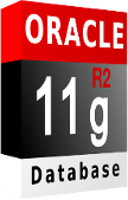
\includegraphics[scale=1]{oracle_11g}
\end{minipage}
\begin{minipage}[c]{0.8\textwidth}
    So wird das Ergebnis in einer Oracle 11g R2 Datenbank dargestellt.
\end{minipage}
\vfil
\begin{minipage}[c]{2cm}
    
\includegraphics[scale=1]{ms_sql}
\end{minipage}
\begin{minipage}[c]{0.8\textwidth}
    So wird das Ergebnis in einem Mircrosoft SQL Server 2008 R2 dargestellt.
\end{minipage}
\vfil
\begin{minipage}[c]{2cm}
    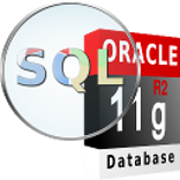
\includegraphics[scale=1]{ms_sql_oracle}
\end{minipage}
\begin{minipage}[c]{0.8\textwidth}
    Oracle und Microsoft SQL Server stellen das Ergebnis auf die gleiche Art und Weise dar.
\end{minipage}
\vfil

Eine solche Abfrage lässt sich nun um beliebige Spalten erweitern.
\begin{lstlisting}[language=oracle_sql,caption={Eine einfache Auswahlabfrage in Oracle},label=sql01_03]
SELECT Vorname, Nachname, Geburtsdatum, SozVersNr
FROM   Mitarbeiter;
        \end{lstlisting}
\clearpage
\begin{center}
    \begin{small}
        \changefont{pcr}{m}{n}
        \tablefirsthead{
            \multicolumn{1}{l}{\textbf{VORNAME}} &
            \multicolumn{1}{l}{\textbf{NACHNAME}} &
            \multicolumn{1}{l}{\textbf{GEBURTSDATUM}} &
            \multicolumn{1}{l}{\textbf{SOZVERSNR}} \\
            \cmidrule(l){1-1}\cmidrule(l){2-2}\cmidrule(l){3-3}\cmidrule(l){4-4}
        }
        %             \tabletail{
        %               \multicolumn{4}{l}{\textbf{100 Zeilen ausgewählt}} \\
        %             }
        \tablelasttail{
            \multicolumn{4}{l}{\textbf{100 Zeilen ausgewählt}} \\
        }
        \begin{msoraclesql}
            \begin{supertabular}{llll}
                Max & Winter & 31.08.88 & D370941F-6CD-6C07977\\
                Sarah & Werner & 03.11.77 & 18FE2247-C53-7EAD1ED\\
                Finn & Seifert & 17.10.85 & C973A840-B92-C5B97CD\\
                Sebastian & Schwarz & 27.06.92 & E8F8587D-CBA-0F28A80\\
                Tim & Sindermann & 11.01.80 & 703838BD-E9C-BD118A6\\
            \end{supertabular}
        \end{msoraclesql}
    \end{small}
\end{center}
\subsection{Der * als Joker}
In verschiedenen Kartenspielen gibt es Karten, die als Joker dienen. Solche \enquote{Universalkarten} können sich, in der richtigen Situation ausgespielt, als sehr nützlich erweisen. Auch in SQL gibt es einen Joker, den Stern *. Er ist immer dann dienlich, wenn man die Spaltenstruktur einer Tabelle nicht kennt oder einfach alle Spalten ausgeben möchte.
\begin{lstlisting}[language=oracle_sql,caption={Der * als Joker},label=sql01_04]
SELECT *
FROM   Bankfiliale;
        \end{lstlisting}
\begin{center}
    \begin{small}
        \changefont{pcr}{m}{n}
        \tablefirsthead{
            \multicolumn{1}{l}{\textbf{BANKFILIALE\_ID}} &
            \multicolumn{1}{l}{\textbf{STRASSE}} &
            \multicolumn{1}{l}{\textbf{HAUSNUMMER}} &
            \multicolumn{1}{l}{\textbf{PLZ}} &
            \multicolumn{1}{l}{\textbf{ORT}} \\
            \cmidrule(l){1-1}\cmidrule(l){2-2}\cmidrule(l){3-3}\cmidrule(l){4-4}\cmidrule(l){5-5}
        }
        \tabletail{
            \multicolumn{5}{l}{\textbf{21 Zeilen ausgewählt}} \\
        }
        \tablelasttail{
            \multicolumn{5}{l}{\textbf{21 Zeilen ausgewählt}} \\
        }
        \begin{msoraclesql}
            \begin{supertabular}{rllll}
                1 & Poststraße & 1 & 06449 & Aschersleben\\
                2 & Markt & 5 & 06449 & Aschersleben\\
                3 & Goethestraße & 4 & 39240 & Calbe\\
                4 & Lessingstraße & 1 & 06406 & Bernburg\\
                5 & Schillerstraße & 7 & 39240 & Barby\\
                6 & Kirchstraße & 8 & 39444 & Hecklingen\\
                7 & Ringstraße & 10 & 06420 & Könnern\\
            \end{supertabular}
        \end{msoraclesql}
    \end{small}
\end{center}
\begin{merke}
    Der Stern * dient, in der SELECT-Liste einer Auswahlabfrage, als Platzhalter, stellvertretend für alle Spalten einer Tabelle.
\end{merke}
Sollen alle Spalten, bis auf eine einzige angezeigt werden, kann der Stern leider nicht weiterhelfen. Eine Formulierung wie \enquote{* -1} ist nicht möglich. In einem solchen Fall müssen alle Spalten, bis auf die betreffende angegeben werden.
\subsection{Arithmetische Ausdrücke}
SQL ist, wie viele andere Programmiersprachen auch, in der Lage arithmetische Ausdrücke zu berechnen. Diese können nicht nur in der SELECT-Liste des SQL-Statements, sondern auch in verschiedenen anderen Klauseln, vorkommen. Die Syntax solcher Ausdrücke unterscheidet sich in Oracle und SQL Server nicht.
\begin{center}
    \tablecaption{Arithmetische Operatoren in Oracle und SQL Server}
    \tablefirsthead{
        \multicolumn{1}{c}{\textbf{(Operator)}} &
        \multicolumn{1}{c}{\textbf{(Bedeutung)}} \\
        \hline
    }
    \tabletail{
        \hline
    }
    \tablelasttail {
        \hline
    }
    \begin{supertabular}{ll}
        + & Addition \\
        - & Subtraktion \\
        * & Multiplikation \\
        / & Division \\
        \%& Modulo (Nur SQL-Server)\\
        . & Dezimaltrennzeichen\\
    \end{supertabular}
\end{center}

\beispiel{sql01_05} zeigt ein einfaches Anwendungsbeispiel. Für die Entscheidung über die Gehaltserhöhung der Mitarbeiter, ist es notwendig, im Vorfeld eine Auswertung zu erstellen, die zeigt, wie sich die Erhöhung von 2,5 \% auf die aktuellen Gehälter auswirkt.

\begin{lstlisting}[language=oracle_sql,caption={Arithmetische Ausdrücke in SQL},label=sql01_05]
SELECT Mitarbeiter_ID, Nachname, Gehalt, Gehalt * 1.025
FROM   Mitarbeiter;
        \end{lstlisting}
\begin{center}
    \begin{small}
        \changefont{pcr}{m}{n}
        \tablefirsthead {
            \multicolumn{1}{r}{\textbf{MITARBEITER\_ID}} &
            \multicolumn{1}{l}{\textbf{NACHNAME}} &
            \multicolumn{1}{r}{\textbf{GEHALT}} &
            \multicolumn{1}{r}{\textbf{GEHALT*1.025}} \\
            \cmidrule(r){1-1}\cmidrule(r){2-2}\cmidrule(r){3-3}\cmidrule(r){4-4}
        }
        \tablehead{}
        \tabletail {
            \multicolumn{4}{l}{\textbf{100 Zeilen ausgewählt}} \\
        }
        \tablelasttail {
            \multicolumn{4}{l}{\textbf{100 Zeilen ausgewählt}} \\
        }
        \begin{oraclesql}
            \begin{supertabular}{rlrr}
                1 & Winter & 88000 & 90200 \\
                2 & Werner & 50000 & 51250 \\
                3 & Seifert & 50000 & 51250 \\
                4 & Schwarz & 30000 & 30750 \\
                5 & Sindermann & 30000 & 30750 \\
                6 & Müller & 30000 & 30750 \\
            \end{supertabular}
        \end{oraclesql}
    \end{small}
\end{center}
\clearpage
\begin{center}
    \begin{small}
        \changefont{pcr}{m}{n}
        \tablefirsthead {
            \multicolumn{1}{r}{\textbf{MITARBEITER\_ID}} &
            \multicolumn{1}{l}{\textbf{NACHNAME}} &
            \multicolumn{1}{r}{\textbf{GEHALT}} &
            \multicolumn{1}{r}{\textbf{GEHALT*1.025}} \\
            \cmidrule(r){1-1}\cmidrule(r){2-2}\cmidrule(r){3-3}\cmidrule(r){4-4}
        }
        \tablehead{}
        \tabletail {
            \multicolumn{4}{l}{\textbf{100 Zeilen ausgewählt}} \\
        }
        \tablelasttail {
            \multicolumn{4}{l}{\textbf{100 Zeilen ausgewählt}} \\
        }
        \begin{mssql}
            \begin{supertabular}{llll}
                1 & Winter & 88000 & 90200 \\
                2 & Werner & 50000 & 51250 \\
                3 & Seifert & 50000 & 51250 \\
                4 & Schwarz & 30000 & 30750 \\
                5 & Sindermann & 30000 & 30750 \\
                6 & Müller & 30000 & 30750 \\
            \end{supertabular}
        \end{mssql}
    \end{small}
\end{center}
\begin{merke}
    Oracle und SQL Server unterscheiden sich in der Anzeige von numerischen Werten. Oracle stellt Zahlen immer rechtsbündig dar. SQL Server zeigt dagegen alle Werte linksbündig an.
\end{merke}
\subsection{NULL Werte}
\label{nullvalues}
Es kommt vor, dass nicht immer alle Attribute eines Datensatzes befüllt sind, d. h. einige Attribute haben keinen Attributwert. Dies kann aus zwei Gründen der Fall sein:
\begin{itemize}
    \item Der Wert eines Attributes ist zum Zeitpunkt der Eingabe des Datensatzes nicht bekannt (z. B. der Vorname einer Person ist nicht bekannt).
    \item Der Wert eines Attributs steht zum Zeitpunkt der Eingabe des Datensatzes noch nicht fest (z. B. das Sterbedatum einer Person bei der Erstellung der Geburtsurkunde).
\end{itemize}
\begin{merke}
    Ein NULL Wert steht immer für einen unbekannten Wert und ist nicht mit der natürlichen Zahl 0 zu verwechseln.
\end{merke}
NULL Werte haben insbesondere bei der Verwendung arithmetischer Ausdrücke eine große Bedeutung. Um dies zu demonstrieren, soll für alle Mitarbeiter deren Monatsgehalt berechnet werden. Dieses setzt sich aus dem Grundgehalt (Spalte \identifier{gehalt}) und einer Provision (Spalten \identifier{provision})zusammen. Da nicht jeder Mitarbeiter eine Provision erhält, existieren NULL Werte in der Tabelle \identifier{Mitarbeiter}.
\begin{lstlisting}[language=oracle_sql,caption={NULL in arithmetischen Ausdrücken},label=sql01_06]
SELECT Vorname, Nachname, Gehalt + Gehalt / 100 * Provision
FROM   Mitarbeiter;
        \end{lstlisting}
\clearpage
\begin{center}
    \begin{small}
        \changefont{pcr}{m}{n}
        \tablefirsthead {
            \multicolumn{1}{l}{\textbf{VORNAME}} &
            \multicolumn{1}{l}{\textbf{NACHNAME}} &
            \multicolumn{1}{r}{\textbf{GEHALT+GEHALT/100*PROVISION}} \\
            \cmidrule(l){1-1}\cmidrule(l){2-2}\cmidrule(l){3-3}
        }
        \tablehead{}
        \tabletail {
            \multicolumn{3}{l}{\textbf{100 Zeilen ausgewählt}} \\
        }
        \tablelasttail {
            \multicolumn{3}{l}{\textbf{100 Zeilen ausgewählt}} \\
        }
        \begin{oraclesql}
            \begin{supertabular}{llr}
                Max & Winter &  \\
                Sarah & Werner &  \\
                ... & ... & ... \\
                Johannes & Lehmann & 2400 \\
                Louis & Schmitz & 2500 \\
                Martin & Schacke & 1200 \\
            \end{supertabular}
        \end{oraclesql}
    \end{small}
\end{center}
\begin{merke}
    Einige Mitarbeiter erhalten keine Provision. Oracle und SQL Server unterscheiden sich bei der Anzeige der NULL Werte. Oracle zeigt für NULL Werte nichts an. SQL Server zeigt die Zeichenkette NULL an.
\end{merke}
Und hier das Ergebnis für den MS SQL Server.
\begin{center}
    \begin{small}
        \changefont{pcr}{m}{n}
        \tablefirsthead {
            \multicolumn{1}{l}{\textbf{VORNAME}} &
            \multicolumn{1}{l}{\textbf{NACHNAME}} &
            \multicolumn{1}{r}{\textbf{(Kein Spaltenname)}} \\
            \cmidrule(l){1-1}\cmidrule(l){2-2}\cmidrule(l){3-3}
        }
        \tablehead{}
        \tabletail {
            \multicolumn{3}{l}{\textbf{100 Zeilen ausgewählt}} \\
        }
        \tablelasttail {
            \multicolumn{3}{l}{\textbf{100 Zeilen ausgewählt}} \\
        }
        \begin{mssql}
            \begin{supertabular}{llr}
                Max & Winter &  NULL \\
                Sarah & Werner &  NULL \\
                Finn & Seifert &  NULL \\
                ... & ... & ... \\
                Johannes & Lehmann & 2400 \\
                Louis & Schmitz & 2500 \\
                Marie & Kipp &  NULL \\
                Amelie & Krüger &  NULL \\
                Martin & Schacke & 1200 \\
                ... & ... & ... \\
            \end{supertabular}
        \end{mssql}
    \end{small}
\end{center}
\begin{merke}
    Jeder arithmetische Ausdruck, in dem ein NULL Wert als Operand vorkommt, hat als Ergebnis den Wert NULL.
\end{merke}
\subsection{Verkettung von Zeichenketten}
In manchen Fällen ist es notwendig, die Ausgabe einzelner Spalten miteinander zu verbinden. Dieser Vorgang wird als Konkatenation\footnote{Verkettung von Zeichen oder Zeichenketten} bezeichnet. Hierfür kennt Oracle den Operator \textbardbl{} und SQL Server den Operator +.

\beispiel{sql01_05} wird nun dahingehend erweitert, dass die Gehaltserhöhung als Bericht angezeigt wird. Für jeden Mitarbeiter muss eine Zeile der Form \enquote{AAA hat ein Gehalt von XXX EUR und soll YYY EUR erhalten.}
\begin{lstlisting}[language=oracle_sql,caption={Verkettung von Zeichenketten in Oracle},label=sql01_07]
SELECT Nachname || ' hat ein Gehalt von ' || Gehalt ||
       ' EUR und soll ' || (Gehalt * 1.025) ||
       ' EUR erhalten.'
FROM   Mitarbeiter;
        \end{lstlisting}
\begin{center}
    \begin{small}
        \changefont{pcr}{m}{n}
        \tablefirsthead {
            \multicolumn{1}{l}{\textbf{NACHNAME||'HATEINGEHALTVON'||GEHALT||'EURUNDSOL...'}} \\
            \cmidrule(l){1-1}
        }
        \tablehead{}
        \tabletail {
            \multicolumn{1}{l}{\textbf{100 Zeilen ausgewählt}} \\
        }
        \tablelasttail {}
        \begin{oraclesql}
            \begin{supertabular}{l}
                Winter hat ein Gehalt von 88000 EUR und soll 90200 EUR erhalten. \\
                \dots \\
                Lehmann hat ein Gehalt von 2000 EUR und soll 2050 EUR erhalten. \\
                Schmitz hat ein Gehalt von 2000 EUR und soll 2050 EUR erhalten. \\
                Kipp hat ein Gehalt von 2000 EUR und soll 2050 EUR erhalten. \\
                \dots \\
            \end{supertabular}
        \end{oraclesql}
    \end{small}
\end{center}
\begin{lstlisting}[language=ms_sql,caption={Verkettung von Zeichenketten in SQL Server},label=sql01_08]
SELECT Nachname + ' hat ein Gehalt von '+ CAST(Gehalt AS VARCHAR(15)) +
       ' EUR und soll ' +
       CAST(Gehalt * 1.025 AS VARCHAR(15)) + ' erhalten.'
FROM   Mitarbeiter;
        \end{lstlisting}
\begin{center}
    \begin{small}
        \changefont{pcr}{m}{n}
        \tablefirsthead {
            \multicolumn{1}{l}{\textbf{(Kein Spaltenname)}} \\
            \cmidrule(l){1-1}
        }
        \tablehead{}
        \tabletail {
            \multicolumn{1}{l}{\textbf{100 Zeilen ausgewählt}} \\
        }
        \tablelasttail {
            \multicolumn{1}{l}{\textbf{100 Zeilen ausgewählt}} \\
        }
        \begin{mssql}
            \begin{supertabular}{l}
                Winter hat ein Gehalt von 88000 EUR und soll 90200 EUR erhalten. \\
                ... \\
                Lehmann hat ein Gehalt von 2000.00 EUR und soll ...  \\
                Schmitz hat ein Gehalt von 2000.00 EUR und soll ...  \\
                ... \\
                Schacke hat ein Gehalt von 1000.00 EUR und soll 1025 EUR erhalten. \\
                ... \\
            \end{supertabular}
        \end{mssql}
    \end{small}
\end{center}
An \beispiel{sql01_07} und \beispiel{sql01_08} sieht man sehr gut die unterschiedliche Reaktionsweise beider Datenbank Management Systeme. Oracle ist ohne weiteres in der Lage, Daten unterschiedlichen Typs (Zeichenketten, Zahl, Datumswerte, usw.) miteinander zu verknüpfen.

Bei Microsoft SQL Server ist dies nicht der Fall. Hier muss ein Vorgriff auf spätere Kapitel erfolgen. Der Zahlenwert der aus der Berechnung \textit{gehalt * 1.025} resultiert, muss explizit in eine Zeichenkette umgewandelt werden, bevor die Verkettung funktioniert.
\subsection{Spaltenaliasnamen}
Bei der Anzeige des Ergebnisses einer Auswahlabfrage wird für jede Spalte eine Überschrift erzeugt. Oracle und Microsoft SQL Server sind sich dabei in sofern einig, als dass für die Spaltenüberschriften die Spaltenbezeichner der Tabellenspalten genutzt werden. Wird aber in der \languageorasql{SELECT}-Liste eine Konstante, eine Funktion oder ein anderer Ausdruck genutzt, scheiden sich die Geister. SQL Server zeigt in so einem Falle einfach gar keine Überschrift an, während Oracle einen Teil des Ausdrucks als Überschrift nutzt. Dieses Verhalten ist in den vorangegangenen Beispielen an einigen Stellen zu sehen.

Der SQL-Standard erlaubt es dieses Verhalten zu beeinflussen und manuell eine Spaltenüberschrift, einen sogenannten \enquote{Spaltenaliasnamen}, zu vergeben. Dies funktioniert im Falle von Oracle und SQL Server auf die gleiche Art und Weise, da sich hier beide an den Standard halten.
\begin{lstlisting}[language=oracle_sql,caption={Vergabe eines Spaltenaliasnamen},label=sql01_09]
SELECT Vorname, Nachname, Gehalt + Gehalt / 100 * Provision AS "Neues Gehalt"
FROM   Mitarbeiter;
        \end{lstlisting}
\begin{center}
    \begin{small}
        \changefont{pcr}{m}{n}
        \tablefirsthead {
            \multicolumn{1}{l}{\textbf{VORNAME}} &
            \multicolumn{1}{l}{\textbf{NACHNAME}} &
            \multicolumn{1}{r}{\textbf{Neues Gehalt}} \\
            \cmidrule(l){1-1}\cmidrule(l){2-2}\cmidrule(l){3-3}
        }
        \tablehead{}
        \tabletail {
            \multicolumn{3}{l}{\textbf{100 Zeilen ausgewählt}} \\
        }
        \tablelasttail {
            \multicolumn{3}{l}{\textbf{100 Zeilen ausgewählt}} \\
        }
        \begin{msoraclesql}
            \begin{supertabular}{llr}
                ... & ... & ... \\
                Johannes & Lehmann & 2400 \\
                Louis & Schmitz & 2500 \\
                Marie & Kipp &  \\
                Amelie & Krüger &  \\
                Stefan & Beck &  \\
                Martin & Schacke & 1200 \\
                ... & ... & ... \\
            \end{supertabular}
        \end{msoraclesql}
    \end{small}
\end{center}

Der ANSI SQL-Standard sieht vier verschiedene Möglichkeiten zur Angabe eines Spaltenaliasnamen vor:
\begin{itemize}
    \item \languageorasql{[Ausdruck] AS "Spaltenaliasname"}
    \item \languageorasql{[Ausdruck] "Spaltenaliasname"}
    \item \languageorasql{[Ausdruck] Spaltenaliasname}
    \item \languageorasql{[Ausdruck] AS Spaltenaliasname}
\end{itemize}
Oracle und MS SQL Server unterstützen alle vier Varianten. Die Angabe von Anführungszeichen ist nur dann notwendig, wenn im Spaltenaliasnamen Sonderzeichen oder Leerzeichen vorkommen.
\begin{merke}
    Oracle wandelt einen Spaltenaliasnamen automatisch in Großbuchstaben um, es sei den, er wird in Anführungszeichen eingeschlossen.
\end{merke}
\section{Einige Konventionen zu SQL}
Um die Lesbarkeit von SQL-Statements zu verbessern werden an dieser Stelle einige Konventionen genannt, die im praktischen Umgang mit SQL eingehalten werden sollten.
\begin{itemize}
    \item Da SQL-Anweisungen mehrzeilig sein können erhält jede Klausel (SELECT, FROM, usw.) eine eigene Zeile.
    \item SQL ist nicht casesensitiv, d. h. Groß- und Kleinschreibung ist nicht relevant. Zur Verbesserung der Lesbarkeit sollten Schlüsselwörter groß geschrieben werden. Beispiele hierfür sind im gesamten Skript zu finden.
    \item Verwenden Sie Einrückungen zur Verbesserung der Lesbarkeit.
          \begin{lstlisting}[language=ms_sql,caption={So nicht!},label=sql01_10]
SELECT Nachname + ' hat ein Gehalt von  '+
CAST(Gehalt AS VARCHAR(15)) +
' EUR und soll ' +
CAST(Gehalt + Gehalt / 100 * Provision AS VARCHAR(15)) + ' erhalten.'
FROM   Mitarbeiter;
          \end{lstlisting}
          \begin{lstlisting}[language=ms_sql,caption={Viel besser lesbar!},label=sql_01_11]
SELECT Nachname + ' hat ein Gehalt von  '+ CAST(Gehalt AS VARCHAR(15)) +
       ' EUR und soll ' +
       CAST(Gehalt + Gehalt / 100 * Provision AS VARCHAR(15)) + ' erhalten.'
FROM   Mitarbeiter;
          \end{lstlisting}
    \item Gemä\ss\ SQL-Standard muss jedes SQL-Statement mit einem Semikolon (;) abgeschlossen werden. Anwendungen wie der SQL*Developer, der JDeveloper oder das Management Studio verbergen diesen Sachverhalt jedoch.
\end{itemize}
\begin{merke}
    In SQL*Plus muss jedes SQL-Statement mit ; oder / abgeschlossen werden!
\end{merke}
